% ====================================================================
%+
% SECTION:
%    SolarSystem_PHA.tex
%
% CHAPTER:
%    solarsystem.tex
%
% ELEVATOR PITCH:
%    Discovery of PHAs in particular. Discussion of wider 'impacts'.
%
%-
% ====================================================================

\section{Discovery of Potentially Hazardous Asteroids}
\def\secname{\chpname:phas}\label{sec:\secname}

\credit{ivezic},
\credit{rhiannonlynne}.

The U.S. Congress has given a mandate to NASA to implement a
Near-Earth Object (NEO) Survey program to detect, track, catalog, and
characterize the physical characteristics of near-Earth objects equal
to or greater than 140 meters in diameter\footnote{See
\url{http://www.gpo.gov/fdsys/pkg/PLAW-109publ155/pdf/PLAW-109publ155.pdf}}. The
goal is to achieve a completeness of 90\%. In recent practice, adopted
here, the completeness is evaluated for a subset of NEOs called
Potentially Hazardous Asteroids\footnote{Potentially Hazardous
Asteroids (PHAs) are defined as asteroids with a minimum orbit
intersection distance (MOID) of 0.05 AU or less.} (PHA), with
H$\le$22, where H is the absolute magnitude\footnote{Absolute
magnitude is the magnitude that an asteroid would have at a distance
of 1 AU from the Sun and from the Earth, viewed at zero phase
angle. This is an impossible configuration, of course, but the
definition is motivated by desire to separate asteroid physical
characteristics from the observing configuration.} in the Johnson's V
band.

The discovery criteria for PHAs follows the same guidelines and metrics found in the previous
section, \ref{sec:solarsystem:discovery}, but is worth discussing
separately to focus on its main figure
of merit - completeness for PHAs with H$\le$22 magnitudes.

% --------------------------------------------------------------------

\subsection{Target measurements and discoveries}
\label{sec:\secname:targets}

Using the same range of discovery criteria as in the previous section,
\ref{sec:solarsystem:discovery}, we can look at the differential and
cumulative completeness for a population of PHAs. For this sample of
PHAs, we simply pulled the orbits of the brightest (D$>$1~km)
$\sim1500$ PHAs from the Minor Planet Center record. These orbits were
then cloned over a range of $H$ values to evaluate the chances of
discovery for that orbit at each of those $H$ values. The differential
completeness as a function of $H$ is then simply the fraction of
objects which receive at least one set of observations which meet the
discovery criteria during the course of the survey. The cumulative
completeness is similar, but integrated over $H$ by assuming an $H$
distribution with a power-law index of $\alpha=0.3$. Both
differential and cumulative completeness are relevant metrics: the
former provides more insight in the behavior of a particular
simulation, while the latter is a metric given to NASA by the U.S.
Congress. 

To match the NEO mandate, the cumulative completeness at $H$=22 can be
used as a figure of merit.

% --------------------------------------------------------------------

\subsection{Metrics}
\label{sec:\secname:metrics}

The metrics used here are the same as in
\ref{sec:solarsystem:discovery}, although run with different input populations.

% --------------------------------------------------------------------

\subsection{OpSim Analysis}
\label{sec:\secname:analysis}

The differential and cumulative completeness for the baseline survey,
\opsimdbref{db:baseCadence}, at a range of years is shown in
\autoref{fig:baselinePHA}. The baseline cadence achieves a cumulative completeness of 73\% for
H$\le$22 PHAs. The differential completeness at $H$=22 for the same
survey is 58\%, 15\% lower due to increasing completeness toward
smaller $H$ (larger objects). 

%%%%%%%%%%%%%%%%%%%%%%%%%%%
\begin{figure}[th]
%\vskip -1.1in
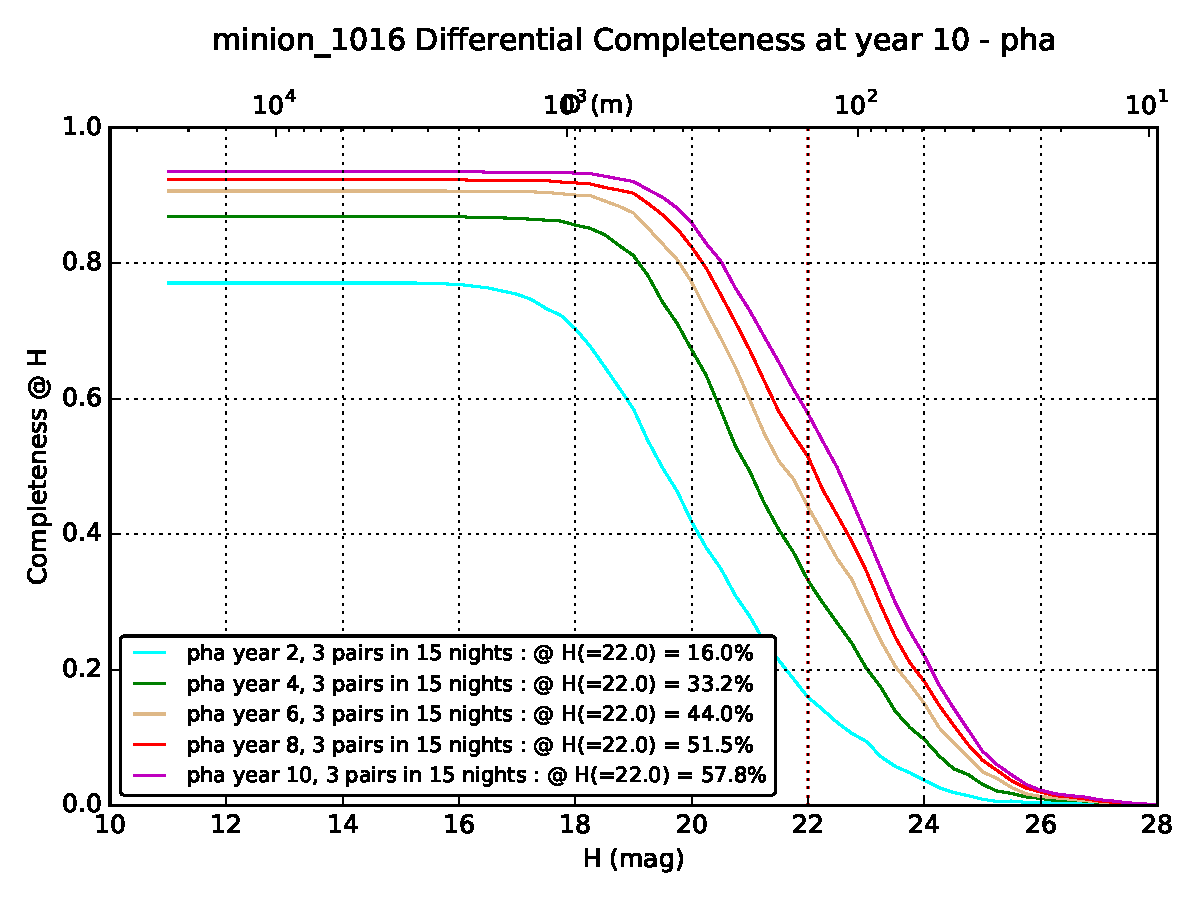
\includegraphics[angle=0,width=0.49\hsize:,clip]{figs/solarsystem/minion_1016_Completeness_2_10_8_6_4_pha_year_3_pairs_in_15_nights_MOOB_ComboMetricVsH}
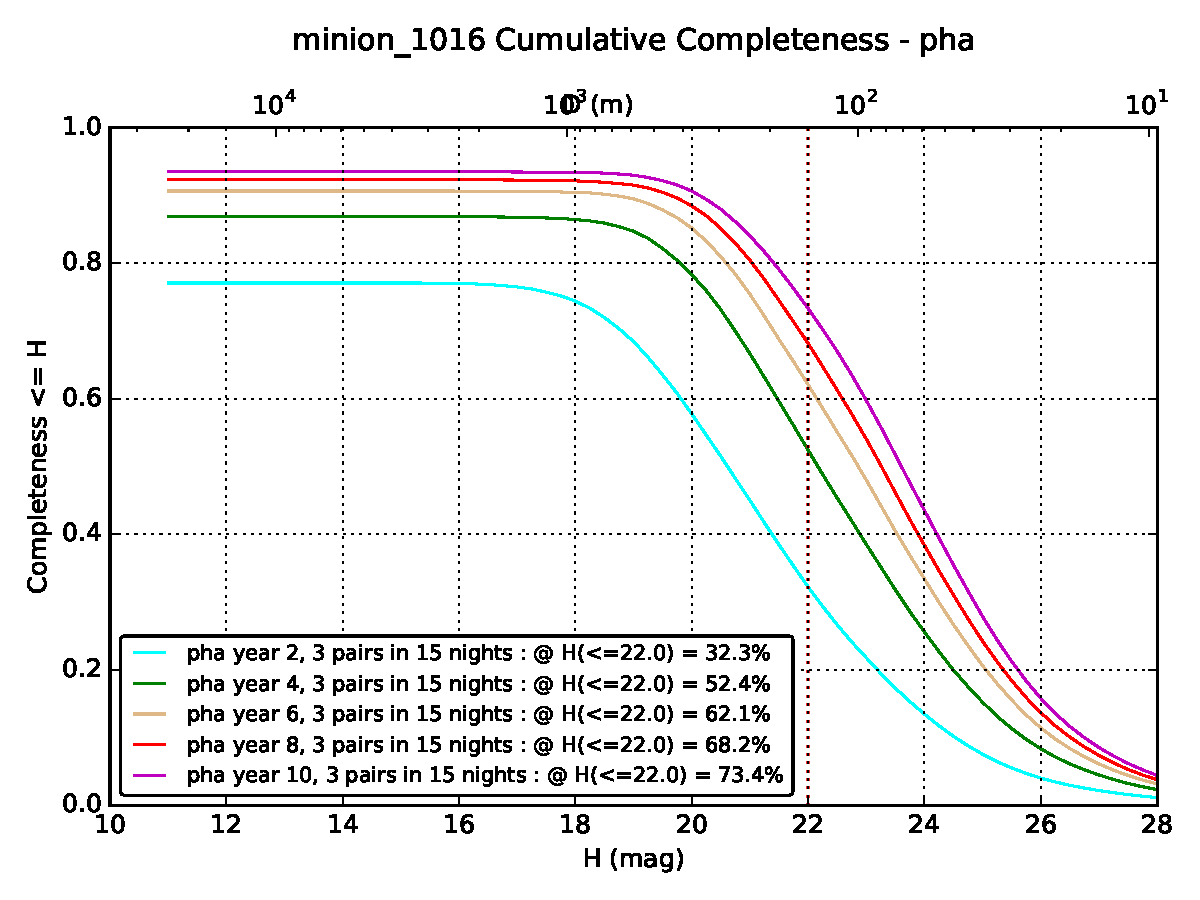
\includegraphics[angle=0,width=0.49\hsize:,clip]{figs/solarsystem/minion_1016_CumulativeCompleteness_2_10_8_6_4_pha_year_3_pairs_in_15_nights_MOOB_ComboMetricVsH}
%\vskip -1.2in
\caption{The PHA completeness for \opsimdbref{db:baseCadence}, as a function of the object's absolute
visual magnitude H on the horizontal axes (left: differential completeness at a given H;
right: cumulative completeness for all objects brighter than a given H).
The cumulative completeness for H$\le$22 NEOs (those with diameters larger than 140m)  for this
simulation is 73\% after 10 years.}
\label{fig:baselinePHA}
\end{figure}
%%%%%%%%%%%%%%%%%%%%%%%%%%%

%%%%%%%%%%%%%%%%%%%%%%%%%%%
\begin{figure}[bh]
%\vskip -1.2in
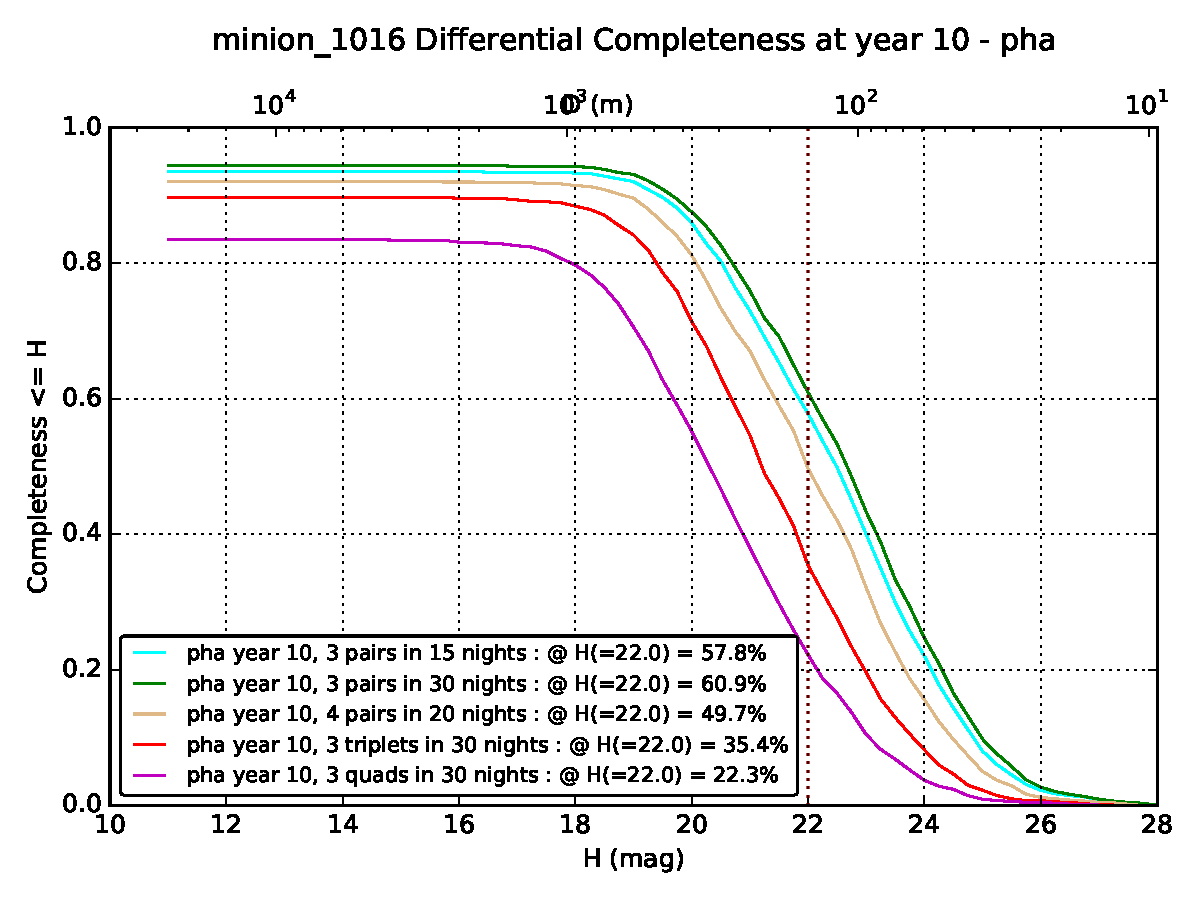
\includegraphics[angle=0,width=0.49\hsize:,clip]{figs/solarsystem/minion_1016_Completeness_3_15_pairs_3_30_pairs_quads_3_30_3_30_triplets_pairs_20_4_nights_in_pha_year_10_MOOB_ComboMetricVsH}
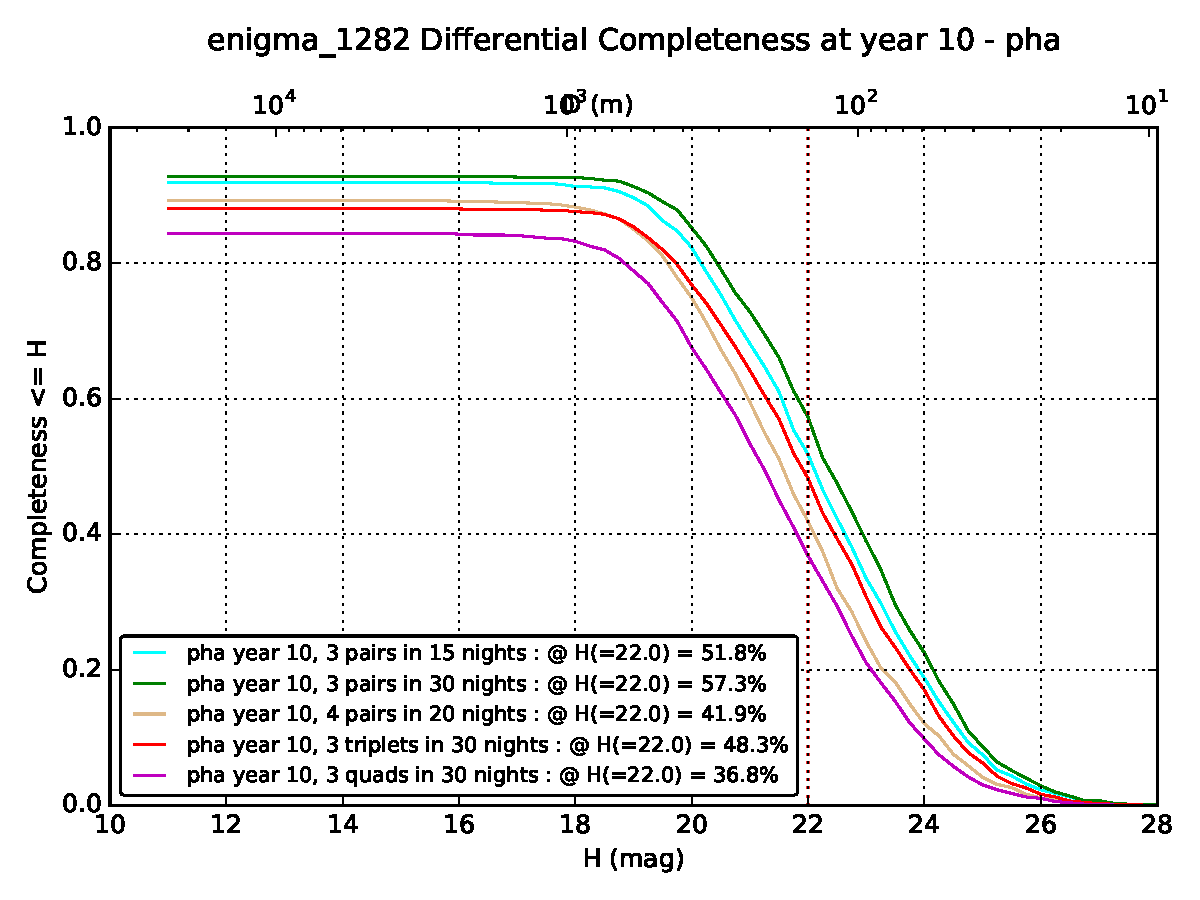
\includegraphics[angle=0,width=0.49\hsize:,clip]{figs/solarsystem/enigma_1282_Completeness_3_15_pairs_3_30_pairs_quads_3_30_3_30_triplets_pairs_20_4_nights_in_pha_year_10_MOOB_ComboMetricVsH}
%\vskip -1.3in
\caption{%
Comparison of the differential PHA completeness for the baseline cadence
\opsimdbref{db:baseCadence}, requesting two detections per night (left), and 
\opsimdbref{db:NEOvisitsWithQuads}, requesting four detections per
night (right). With a discovery criteria of 3 pairs within 15 nights,
both surveys perform roughly similarly; with a discovery criteria of 3
sets of quad visits within 30 nights,
\opsimdbref{db:NEOvisitsWithQuads} performs better (as expected),
although still at a lower completeness level than
\opsimdbref{db:baseCadence} did with the pairs criteria.}
\label{fig:strategiesPHA}
\end{figure}
%%%%%%%%%%%%%%%%%%%%%%%%%%%
 
The differential completeness for a range of discovery criteria, for
both the baseline survey and \opsimdbref{db:NEOwithVisitQuads}, is
shown in \autoref{fig:strategiesPHA}. When the discovery algorithm
requires pairs of visits, the runs have fairly similar PHA
completeness, with \opsimdbref{db:NEOwithVisitQuads} having a
differential completeness about 6\% lower than
\opsimdbref{db:baseCadence}.  When the discovery algorithm requires 4
detections per night, the simulation with quads achieves a
differential completeness of about 15\% higher than the baseline
cadence (as some quads are unintentionally produced by chance, see
\autoref{fig:NvisitStats}).

\begin{table}[h]
\centering
\caption{Differential PHA completeness at $H$=22}
\label{phacompleteness}
\begin{tabular}{l|c|c|c|c}
 & \opsimdbref{db:baseCadence} & \opsimdbref{db:NoVisitPairs} &
                                                                \opsimdbref{db:NEOswithVisitTriplets}
  & \opsimdbref{db:NEOwithVisitQuads} \\

3 pairs in 15 nights & 58 & 51 & 56 & 52 \\
3 pairs in 30 nights & 61 & 56 & 59 & 57 \\
4 pairs in 20 nights & 50 &  41 & 46 & 42 \\
3 triplets in 30 nights & 35 & 33 & 50 & 48 \\
3 quads in 30 nights & 22 & 18 & 19 & 37 \\

\end{tabular}
\end{table}


\begin{table}[h]
\centering
\caption{Cumulative PHA completeness at $H$=22}
\label{phacompleteness}
\begin{tabular}{l|c|c|c|c}
 & \opsimdbref{db:baseCadence} & \opsimdbref{db:NoVisitPairs} &
                                                                \opsimdbref{db:NEOswithVisitTriplets}
  & \opsimdbref{db:NEOwithVisitQuads} \\

3 pairs in 15 nights & 73 & 69 & 71 & 68 \\
3 pairs in 30 nights & 76 & 73 & 74 & 73 \\
4 pairs in 20 nights & 68 & 62 & 64 & 61 \\
3 triplets in 30 nights & 57 & 55 & 66 & 65 \\ 
3 quads in 30 nights & 42 & 37 & 37 & 55 \\

\end{tabular}
\end{table}

\navigationbar
